\chapter{Entropy and Fractal Dimension Approach}

\textit{by Florian Fallenbüchel}\\

This chapter will explain our approach on the classification of the
genre via the entropy and fractal dimension of the song. This approach
is interesting, because it does not consider musical information such as
harmony, melody, beat and tempo, heavily reducing the size of the data
to be processed during training. The entropy is a measure of the
disorder of the signal, indicating the quantity of change of the signal
energy between consecutive parts of the track. The fractal dimension is
a measure of the complexity of the signal, as it indicates the ratio of
the change of detail to the change in scale at which the detail is
measured. This term is mostly used in fractal geometry, as fractals have
infinite lengths between any two points, making them more complex than
their topological dimension, but less complex than the next higher one.
This interdimensionality is given by the fractal dimension.\\

\section{Method}

We follow the work of Goulart \textit{et al.}~\cite{entropy} from 2012,
who used the entropy approach together with combined support vector
machines. They achieved 100\% classification accuracy on a set of 90
songs equally distributed over 3 different genres, with 80-90\% of the
data used for training. We try to extend this method to a larger amount
of classes, combining it with neural networks for classification.\\
For the calculation of the entropy, we need the energy approach of
signal theory, as presented in Elements of Information Theory
\cite{infotheo} by Cover and Thomas. The song is divided into frames of
1024 samples with 50\% overlap between consecutive frames and the
entropy $E$ then is defined as
\begin{equation}
	E = - \sum_{i=0}^{1023} p_{i} \log_{2}(p_{i}),
\end{equation}
with $p_{i}$ being the proportion of the sample energy to the
energy of the whole frame
\begin{equation}
	p_i = \frac{y_i}{\sum_{j=0}^{1023} y_j}.
\end{equation}
\\
\noindent From the now obtained set of entropies of the song we
calculate five features, namely the average entropy, the standard
deviation of the entropies, the maximum and minimum entropy and the
absolute maximum difference of entropies between consecutive frames.
Those are the first five entries of our input vector for the neural
network.\\
For the calculation of the fractal dimension they suggest a box counting
algorithm. The basic principle of these algorithms is to calculate the
number of boxes of different sizes necessary to cover the entire signal.
After that, a linear least squares solution is computed on the logarithm
of the number of boxes and the inverse logarithm of the respective box
size ($\frac{1}{log(boxs)}$). The slope of the resulting curve then
resembles the fractal dimension.\\
For the implementation of the algorithm, we needed to improvise, because
the box counting algorithm Goulart \textit{et al.} used in their work is
described in the book ``Fractal Speech Processin''~\cite{fractal} by
Al-Akaidi, which is not purchasable or accessible through online
libraries at the moment. We therefore adopted the box counting algorithm
presented by Boshoff~\cite{boxcount}, as it promises fast computation
time due to the doubling of the box size during each step. The fractal
dimension is the last element of our input, resulting in a six
dimensional input vector for the neural network. We vectorized all
algorithms, to be able to efficiently process the huge amount of
available data in a short amount of time.

\section{Model}

\begin{figure}[!htb]
	\centering
	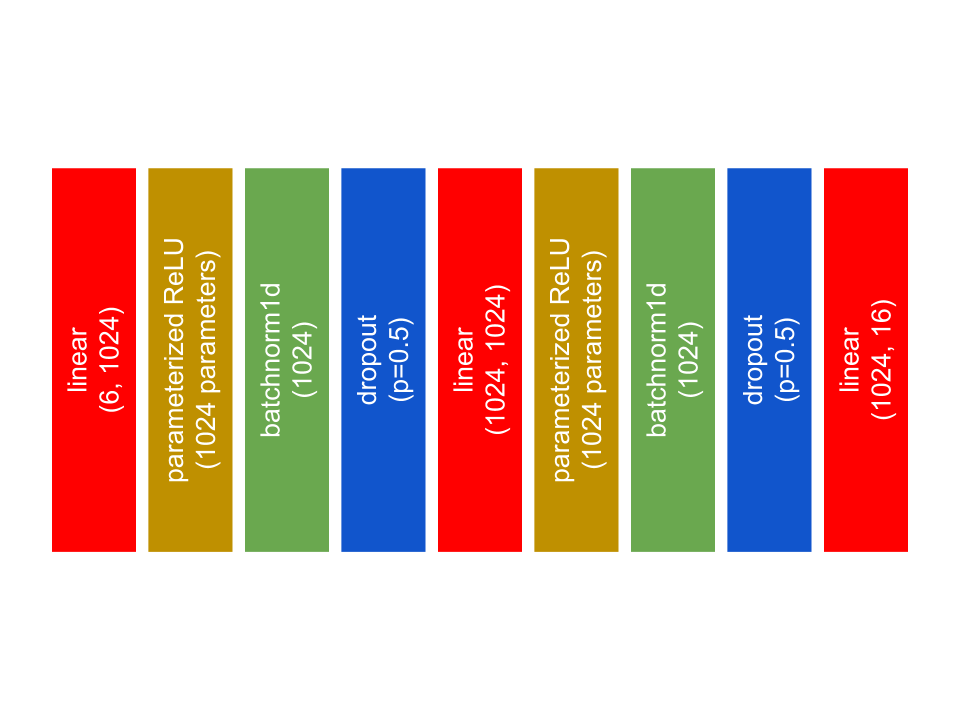
\includegraphics[width=0.65\textwidth]{images/entropymodel.png}
	\caption{Architecture of the neural network used for the classification
	of the 6-dimensional entropy-fractal vector to one of the 16 top
	genres from the dataset.}
	\label{entropymodel}
\end{figure}
As our input data is relatively simple, we can use a conservative
implementation of a neural network for the classification, without the
need for convolutions. Figure~\ref{entropymodel} shows the architecture
of our naive network design. Our hidden layers are of size 1024 and we
chose parameterized ReLUs with a parameter for every connection, as well
as batch normalization and dropout for every layer. Batch normalization
accellerates training, as it reduces the amount by what the hidden unit
values shift around, normalizing the input from previous layers to a
common scale. The dropout layers should stabilize the prediction
accuracy by eliminating parts of the information during training,
reinforcing the remaining neurons. We use Cross Entropy as our loss
function and Adam as our optimizer.

\section{Training}

At first, we used up to 120 seconds of every song for the calculation of
the input vector, as processing the whole song would have taken several
days for the whole dataset on our available hardware. Later we upped
this to 180 seconds, with no obvious changes in prediction accuracy. The
results shown in this chapter are therefore for up to 180 seconds per
song. After the preprocession, the whole set of input vectors is only
around 5 MB of data, allowing for large batch sizes for better gradient
estimation and small training times.

\begin{figure}
	\centering
	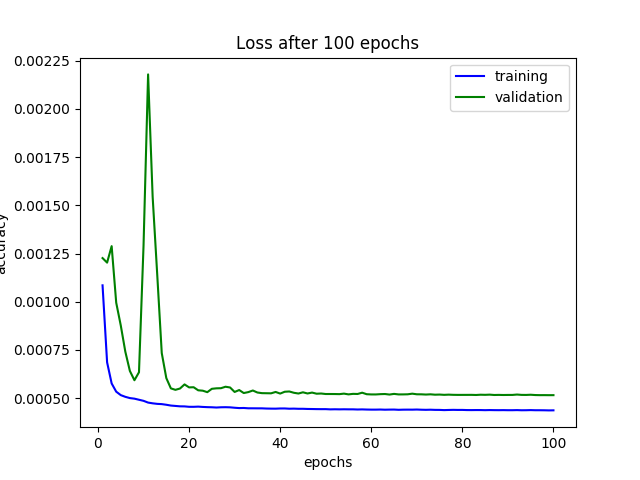
\includegraphics[width=0.45\textwidth]{images/entropyloss.png}
	\centering
	\quad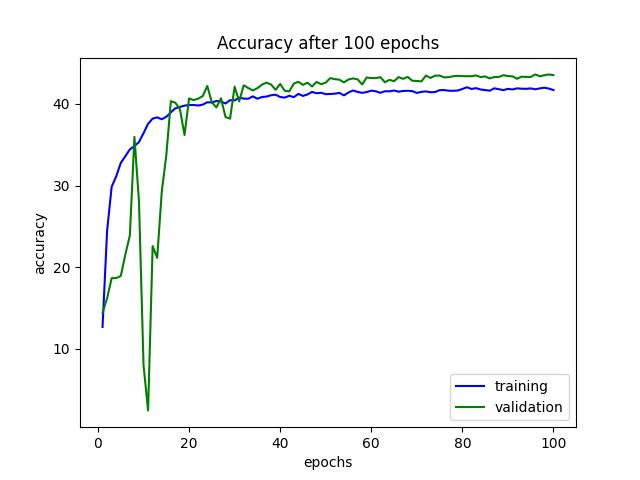
\includegraphics[width=0.45\textwidth]{images/entropyacc.png}
	\caption{Loss and accuracy after 100 epochs with the naive neural
	network implementation.}
	\label{naiveloss}
\end{figure}

Figure~\ref{naiveloss} shows the loss and accuracy of the model over the
first 100 epochs of training. In the beginning, the validation loss and
accuracy are quite unstable, dipping visibly in performance. But, after
a short time, the accuracy is ceils at around 43\%. The loss at this
point is already really low, with no sign of change.

\begin{center}
	\begin{tabular}{ p{0.25\textwidth} p{0.2\textwidth} p{0.2\textwidth} p{0.2\textwidth}}
		Genre & Accuracy & Hits & from Total\\
		\hline
		Instrumental & $0.00\%$ & 0 & 430\\
		Folk & $0.00\%$ & 0 & 558\\
		Country & $0.00\%$ & 0 & 37\\
		Pop & $0.00\%$ & 0 & 481\\
		Hip-Hop & $8.54\%$ & 61 & 714\\
		Electronic & $52.52\%$ & 970 & 1847\\
		International & $0.00\%$ & 0 & 256\\
		Rock & $78.29\%$ & 2226 & 2843\\
		Spoken & $0.00\%$ & 0 & 76\\
		Blues & $0.00\%$ & 0 & 26\\
		Old Time / Historic & $5.31\%$ & 6 & 113\\
		Easy Listening & $0.00\%$ & 0 & 7\\
		Experimental & $45.87\%$ & 993 & 2165\\
		Classical & $34.04\%$ & 80 & 235\\
		Jazz & $0.00\%$ & 0 & 93\\
		Soul-RnB & $0.00\%$ & 0 & 38\\
		\hline
		All & $43,65\%$ & 4330 & 9919\\
	\end{tabular}
	\captionof{table}{Accuracy per class after 100 epochs of training
	with the filtered data set.}
	\label{accperclass}
\end{center}

This might be due to the imbalance of the dataset, as voting for few
classes from big genres might already deliver such a high precision.
Table~\ref{accperclass} gives insight on the accuracy per class- As you
can see, Rock, the biggest genre in the set with around 29\%, also has
the highest precision, indicating that the network learned, that voting
Rock in general seems like a good idea. But also the other two big
genres, Electronic and Experimental, have a relatively high accuracy of
around 45-53\%. More interesting to notice is that Classical music has a
comparatively high accuracy despite its small proportion of the data.
This might be due to the inherent difference of the music to the other
genres, as classical music amongst other things does not tend to have a
beat, probably influencing the standard deviation of the entropy. But
besides Hip-Hop, the fourth biggest part of the set, the network does
not classify any other genre correct at all. These problems are very
likely to be caused by the imbalance, leaving little testing data for
the smaller genres. A more promising approach would have been to start
training on just the two biggest genres and then gradually adding the
smaller genres to the datasets, to see how far this approach can
distinguish music.

\section{Tuning the Hyperparameters of the Network}

To further improve our classification accuracy, we tried to tune the
hyperparameters of our network, like the hidden layer size, the chosen
activation function and learning rate. For this, we used an
implementation of Hypersearch~\cite{hypersearch}, a hyperparameter
optimization tool for neural networks in PyTorch. It embeddes the
Hyperband approach~\cite{hyperband} from Jamieson \textit{et al.}, which
follows the basic principle, that the best configuration for a neural
network is likely to perform in the top half of configurations after a
short amount of iterations. This allows the algorithm to quickly decide
on the capacity of a given neural network configuration.\\
\begin{figure}
	\centering
	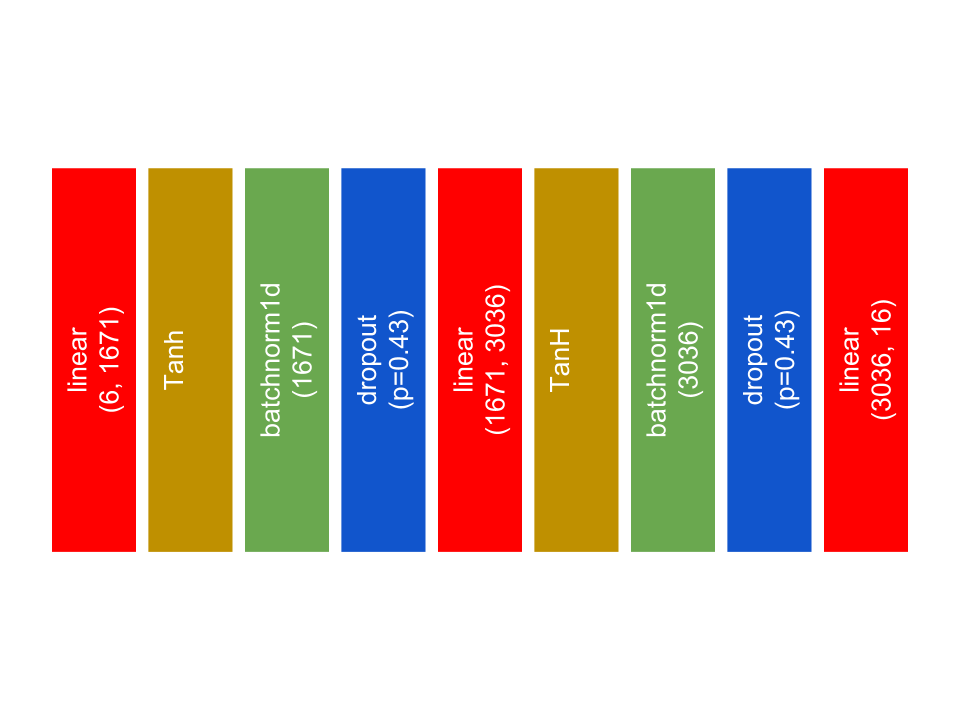
\includegraphics[width=0.65\textwidth]{images/modeltuned.png}
	\caption{Architecture of the model proprosed by Hypersearch after
	evaluating 81 different configurations.}
	\label{modeltuned}
\end{figure}
We tested our network for several activation functions, hidden layer
sizes betwenn 512 and 4096, Adam or SGD as optimizers, different
learning rates and whether dropout and batchnorm are improving the
results if placed behind each layer. The configuration proposed by the
algorithm can be seen in Figure~\ref{modeltuned}. It decided to up the
layer sizes over the naive setup, increasing with the second layer. It
also decided to switch the activation function to tanh. Batch
normalization and dropout seem to support the training as predicted and
therefore stay in the network, just the dropout rate got reduced by a
small amount.\\
\begin{figure}
	\centering
	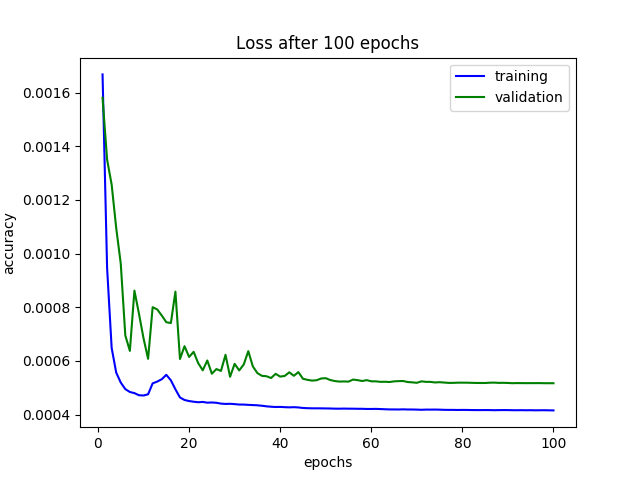
\includegraphics[width=0.45\textwidth]{images/tunedloss.png}
	\centering
	\quad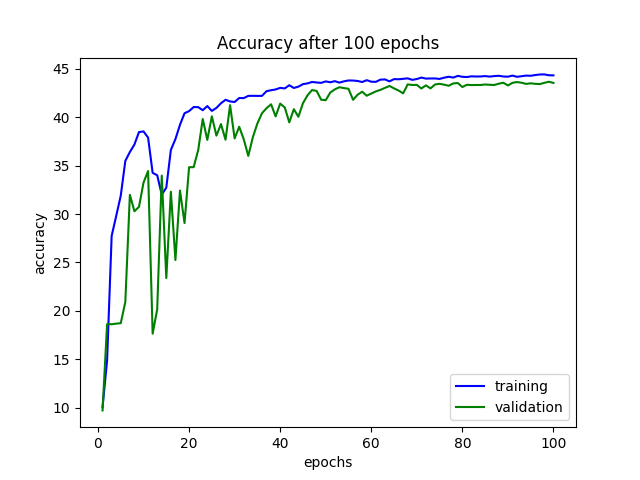
\includegraphics[width=0.45\textwidth]{images/tunedacc.png}
	\caption{Loss and accuracy after 100 epochs with the Hyperparameter
	tuned neural network implementation.}
	\label{tunedloss}
\end{figure}
We used this configuration on the same dataset as in the previous
section, observing the accuracy and loss over the first 100 epochs,
visible in Figure~\ref{tunedloss}. As you can see, the loss and accuracy
is oscillating a little bit less at the start, but then quickly
converges to the same accuracy as the naive approach. Going into detail
in Table~\ref{accperclasstuned} also reveals little difference, but
occasional hits in the smaller genres. These improvements could also be
coincidental and do not necessary represent a better learning process.
The distribution of the data is again most likely the reason for the low
validation accuracy of around 42\%, not allowing the Hypersearch
algorithm to yield any improvement to the training.

\begin{center}
	\begin{tabular}{ p{0.25\textwidth} p{0.2\textwidth} p{0.2\textwidth} p{0.2\textwidth}}
		Genre & Accuracy & Hits & from Total\\
		\hline
		Instrumental & $0.93\%$ & 4 & 430\\
		Folk & $0.00\%$ & 0 & 558\\
		Country & $0.00\%$ & 0 & 37\\
		Pop & $0.00\%$ & 0 & 481\\
		Hip-Hop & $13.17\%$ & 94 & 714\\
		Electronic & $48.78\%$ & 901 & 1847\\
		International & $1.17\%$ & 3 & 256\\
		Rock & $77.03\%$ & 2190 & 2843\\
		Spoken & $1.32\%$ & 1 & 76\\
		Blues & $0.00\%$ & 0 & 26\\
		Old Time / Historic & $0.88\%$ & 1 & 113\\
		Easy Listening & $0.00\%$ & 0 & 7\\
		Experimental & $44.57\%$ & 965 & 2165\\
		Classical & $28.09\%$ & 66 & 235\\
		Jazz & $0.00\%$ & 0 & 93\\
		Soul-RnB & $0.00\%$ & 0 & 38\\
		\hline
		All & $42,60\%$ & 4225 & 9919\\
	\end{tabular}
	\captionof{table}{Accuracy per class after 100 epochs of training
	with the tuned neural network and filtered dataset.}
	\label{accperclasstuned}
\end{center}

\section{Conclusion}

We chose the wrong approach to classify the music via the entropy and
fractal dimension of the songs, as the data set was too imbalanced to
give enough training data for every class. This is an issue, which we
should have realized way earlier, but didnt, impairing the results of
every of our experiments. In the future, we should have started by
trying to distinguish two different genres and then gradually
extending the number of classes. Some literature also suggest to
train individual networks per genre, which only predict if the given
song is their respective genre or not, instead of one network which
has to classify all together.\\
Concerning the method, it is hard to tell its capacity for
classification due to the influenced results. The relatively high
percentages in multiple class accuracies for the larger genres indicate,
that the feature might still incorporate enough information for higher
classification scores. Also, the combination of this feature with, for
example, mel spectograms might deliver really good results. We had the
idea to do a variation of the method, where we calculate the fractal
dimension for every frame of 1024 samples, instead of the whole song and
then average the results for the feature vector. But processing the
whole dataset with this method takes one to two days and we could not
implement this in time.\\
Even though our method looked promising, as it offered efficient
classification on small data (after preprocession), most of our
experiments failed, giving us classification accuracy close to guessing
with 60-70\% of the data being from only three different classes. Still,
we would not discard this method, as some of our results indicate
potential. The small amount of data per song lies near to combine it
with other approaches. With these issues in mind, we could get better
results in the future, not making tremendous mistakes at the basis.
